\section{ShapeLearner - Un plugin de signature}

METIS, en plus d'être un projet de recherche est également le nom du logiciel qui lui est associé. Ce dernier est programmé en JAVA. Il propose une interface à laquelle on peut venir adjoindre de multiples plugins de \textbf{signature}.

Ces derniers se doivent de répondre aux spécifications suivantes :
\begin{itemize}
	\item Être compilé sous forme d'une librairie DLL ou utiliser le langage JAVA.
	\item Exposer une fonction de signature en contexte : \textit{Signature SignInContext(Context);}
	\item Exposer une fonction de comparaison en contexte : \textit{Output MatchInContext(Signature, Context);}
\end{itemize}

\subsection{L'objectif du plugin ShapeLearner}

L'objectif de ce plugin est d'identifier la \textbf{classe} d'un composant mécanique ou d'un assemblage mécanique et ce en prenant en entrée une image 2D de l'objet. Celui-ci doit être le plus robuste possible aux effets d'échelle et à l'angle de prise de vue de l'objet.

Ainsi le plugin doit être capable de donner en sortie le type de pièce ou d'assemblage donné en entrée. \textit{\textbf{Exemple:} Bielle, Piston, Vilebrequin, ...}.

Il est envisageable que l'algorithme retourne soit un seul résultat soit un nombre restreint de résultats avec leur indice de confiance \textit{(par exemple les 3 meilleurs)}. Ce choix pouvant être, par exemple, contrôlé par l'utilisateur. 

\subsection{Le plugin C++ ShapeLearner}

En se basant sur le travail effectué par D. Macrini et al.~\cite{Macrini2002}, nous avons décidé d'adapter le démonstrateur fonctionnel à nos besoins. En effet ce dernier a été publié sous licence Open Source, et a été entièrement programmé en C++.

Dans le soucis de faciliter l'intégration du démonstrateur à notre plugin, nous avons fais le choix d'utiliser nous aussi le langage C++.

\subsubsection{L'architecture logicielle}

Un des points centraux de l'architecture fut de permettre l'utilisation \textbf{\textit{multi-thread}} du démonstrateur fonctionnel mis au point par  D. Macrini et al.~\cite{Macrini2002}. 

Le plugin se compose lui même de plusieurs modules (les modules sont listés en partant de la couche la plus basse jusqu'à la couche supérieure qui est l'interface DLL du plugin) :

\begin{itemize}	
	\item \textbf{Module StandardException: } Ce module a pour rôle de proposer une classe d'exception standard et enrichie pour tout le plugin. Chaque exception générée au sein du programme est gérée de manière unique grâce à cette classe.\\

	\item \textbf{Module CLogger: }``Concurrent Logger'' a pour tâche de réaliser la totalité des actions de \textbf{\textit{logging}} au sein de l'application. Ce module présente une interface entièrement \textbf{\textit{thread-safe}}.\\
	Ce dernier pour notre cas génère quatre fichiers :
	\begin{itemize}
		\item ShapeLearner.Core.log
		\item ShapeLearner.DB.log
		\item ShapeLearner.Error.log
		\item ShapeLearner.Exec.log
	\end{itemize}
	\vspace{3mm}
	
	 \item \textbf{Module GraphDBLib: }Ce module sert de moteur de sauvegarde et de chargement des données depuis et vers les bases de données PostgresSQL associées. Il a été entièrement programmé pour permettre jusqu'à 200 threads concurrents. Il propose une structure objet classique de Graph (Noeuds, Arêtes, ...). Ce dernier gère de manière totalement automatique, transparente et optimisée les interactions avec la base de données. Il est important de préciser que ce module présente deux interfaces. L'une en utilisation classique, l'autre de type SDK permettant de définir des attributs spécifiques ou sous-classes pour chacune des structures classiques du Graph. L'objectif étant de ne pas rendre dépendant le module de la structure spécifique du ShockGraph ou d'un quelconque autre type de Graph. Ce module utilise les deux modules cités plus haut.\\
	 
	 \item \textbf{Module DAGMatcherLib: } Reprise du démonstrateur scientifique de D. Macrini et al.~\cite{Macrini2002}. Modifié afin d'en améliorer les performances, et de permettre l'utilisation multithread. C'est ce dernier qui génère la \textbf{signature} de notre plugin ! C'est le \textbf{cœur} du plugin \textbf{\textit{ShapeLearner}}. Celui se branche directement sur les modules précédents afin de logger les divers évènements lors de la génération de la signature et de sauvegarder le résultat en base de données.\\
	 
	 \item \textbf{Module ShapeLearnerLib: } Module chef d'orchestre, il coordonne les actions et lance la génération des signatures de manière concurrente grâce à l'utilisation d'une threadPool. Ce module est l'unique point d'entrée du plugin. Ce dernier est compilé sous forme de librairie statique (.lib sous windows). C'est ce module qui expose la totalité des fonctionnalités du plugin à destination de pour tout projet visant à la création d'une librairie dynamique ou d'un exécutable utilisant ce plugin.\\
	 
	 \item \textbf{Module ShapeLearnerDLL: } Ce module présente les fonctionnalités du plugin ShapeLearner\- via une interface librairie dynamique (.dll sur windows). Aucune fonctionnalité n'est implémentée dans ce module, il ne fait que transmettre les opérations au module ShapeLearnerLib.\\
\end{itemize} 

\clearpage

Une réel soucis de modularité et non dépendance ascendante des modules entre eux a été la base de notre réflexion. Nous voulions que chaque module du plugin puisse avoir un maximum de sens en dehors de tout contexte. Le but étant de pouvoir réutiliser chacun de ces modules dans une application future si l'occasion se présente. 

Les relations d'interdépendance sont donc à limiter autant que possible. Cependant une relation de dépendance \textbf{\textit{top-down}} est tout à fait possible et même nécessaire. Ainsi le plugin est construit en couches successives. Chaque couche peut interagir avec les couches inférieures, jamais supérieures ou de même niveau.
\vspace{-1cm}

 \begin{figure}[H]
    \centering
    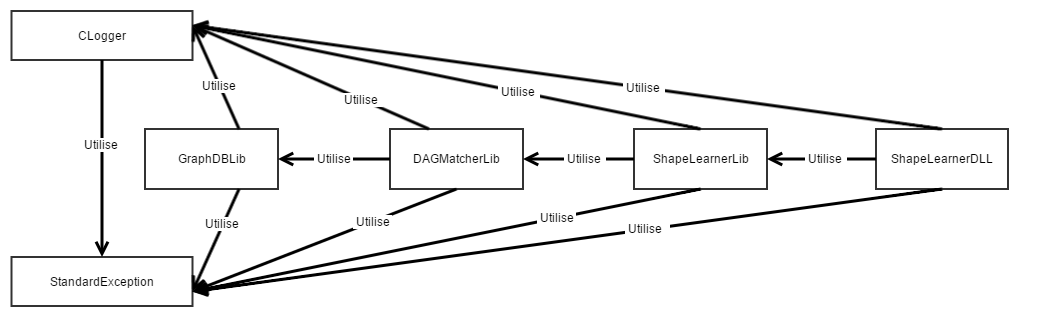
\includegraphics[angle=90,origin=c,height=12.8cm]{shapelearnerplugin_architecture.png}
	\caption{Schéma de l'architecture interne du plugin C++ : ShapeLearner}\label{image.archiShapeLearner} 
\end{figure}

\clearpage

 \begin{figure}[H]
    \centering
    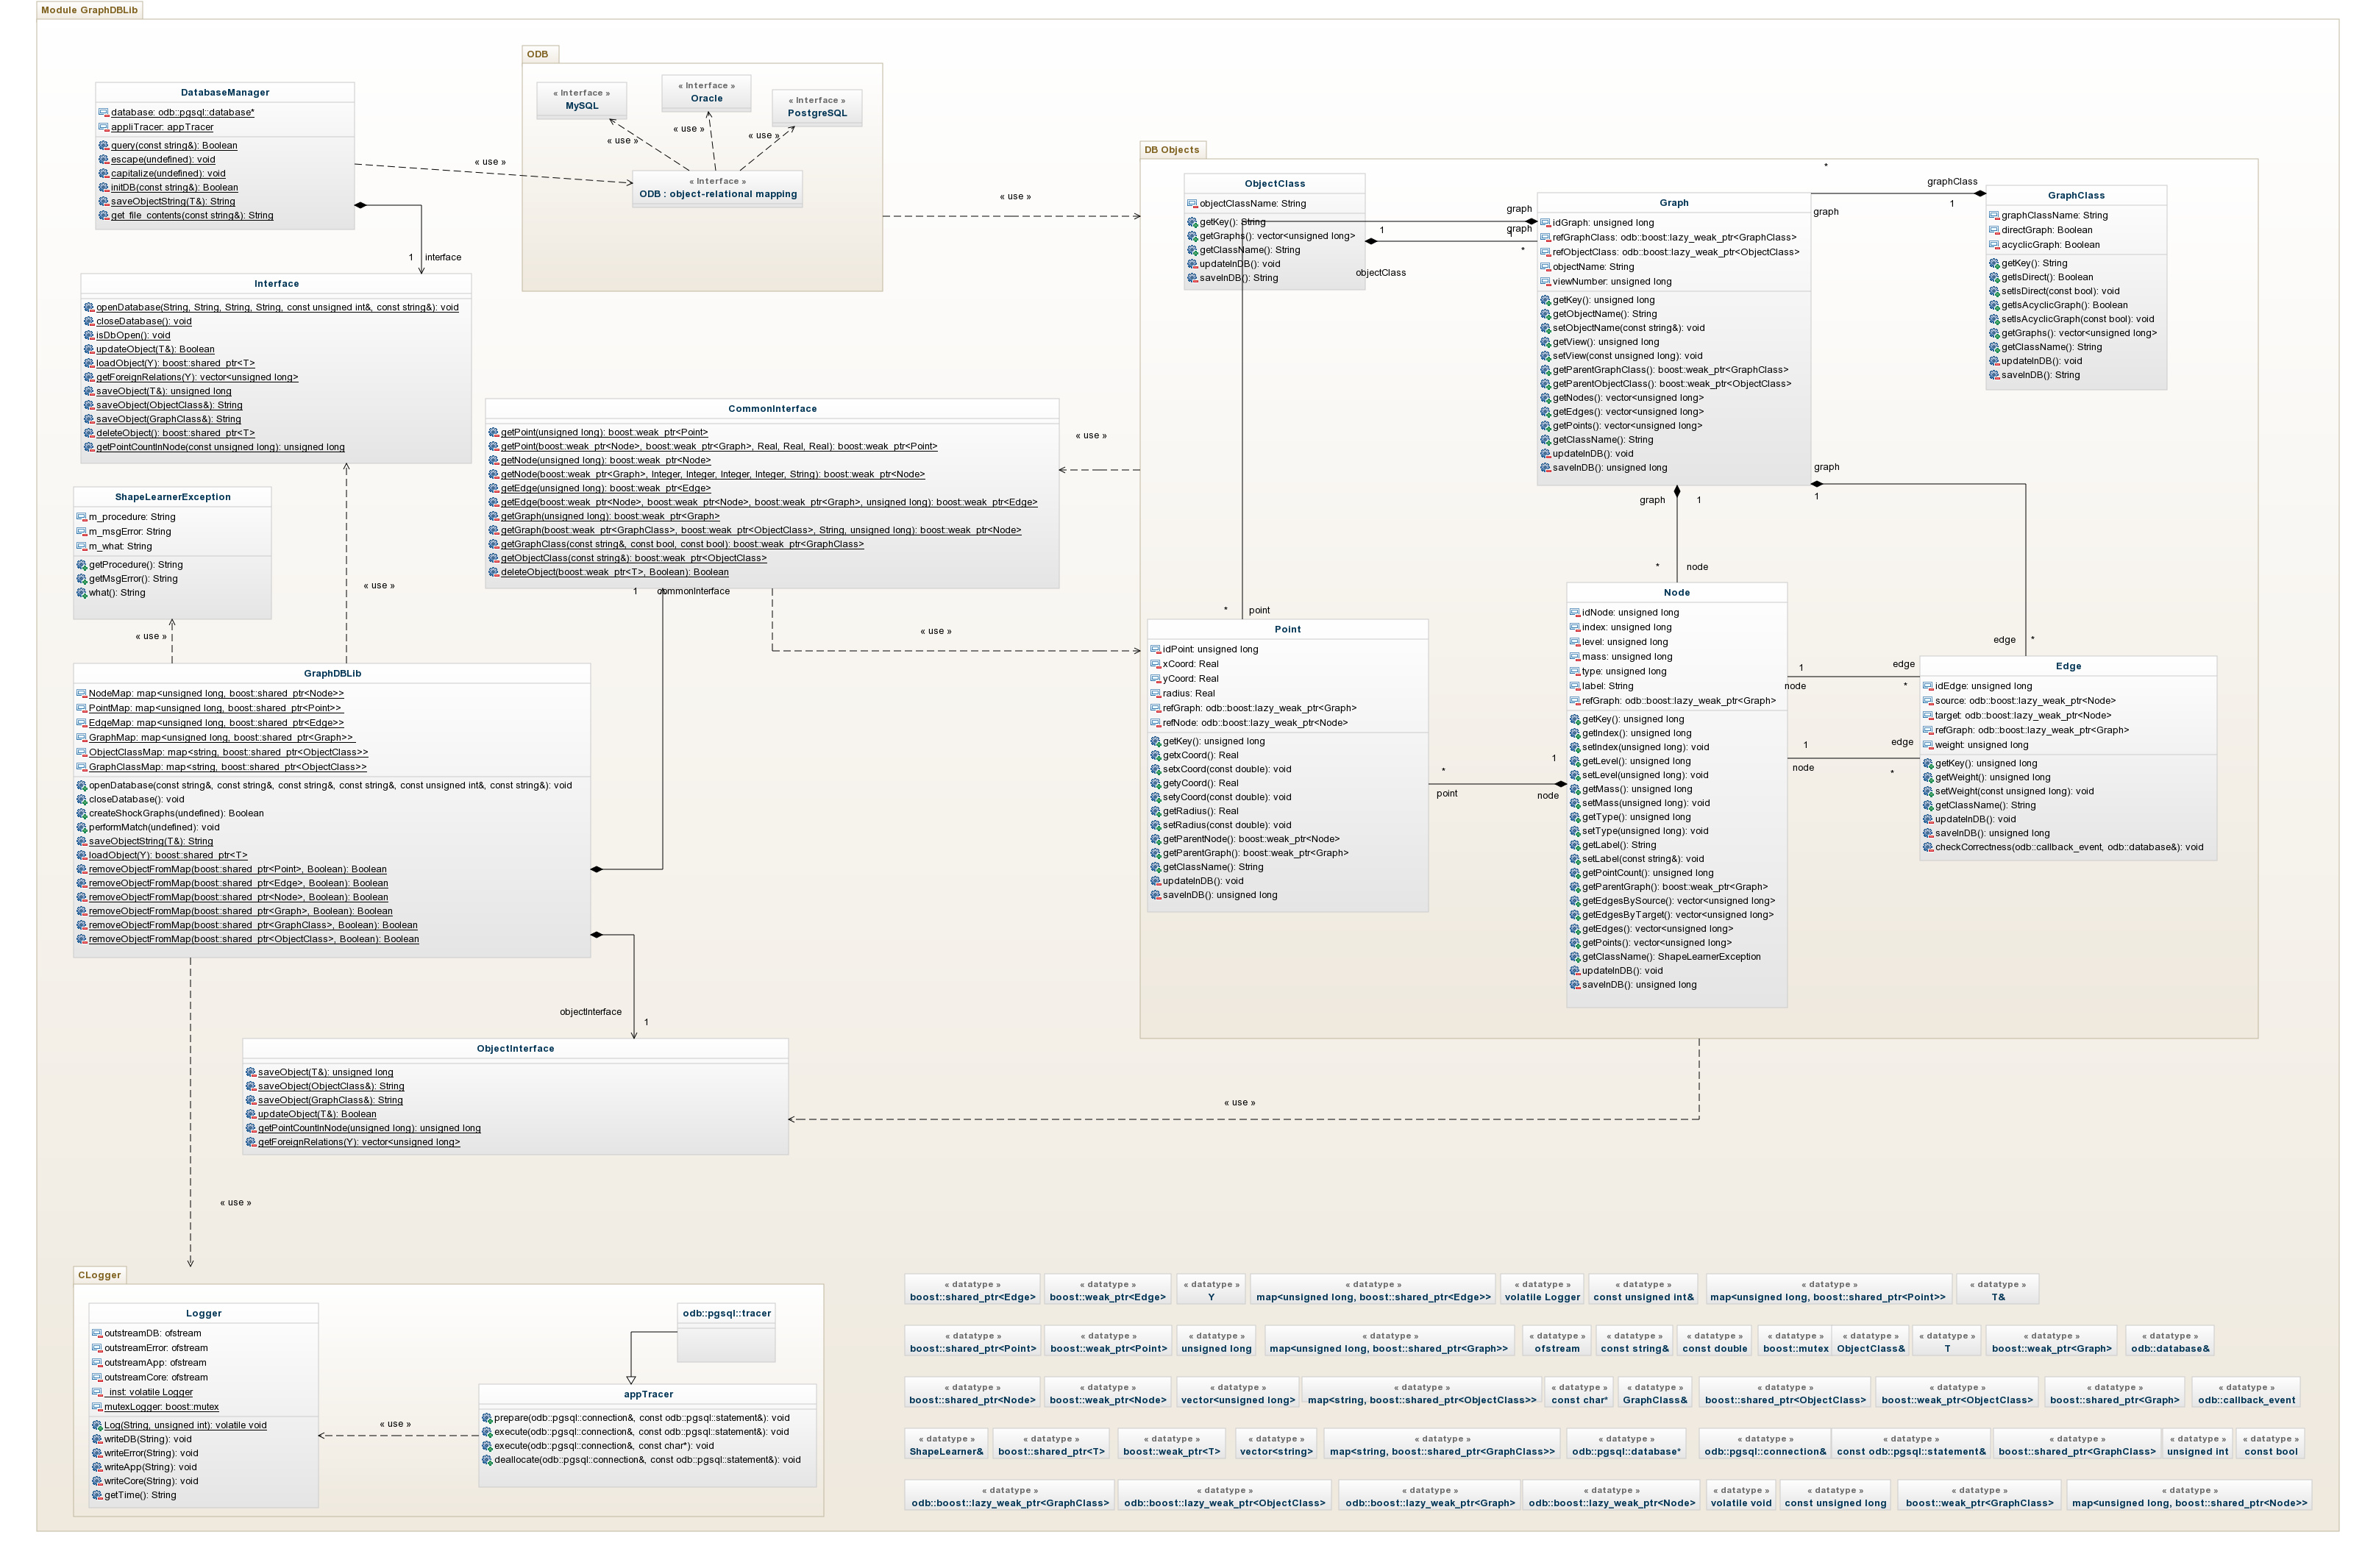
\includegraphics[angle=90,origin=c,height=19.5cm]{ShapeLearner_UML.jpg}
	\caption{Diagramme UML présentant le principe de l'architecture du module GraphDBLib}\label{image.UMLGraphDBLib} 
\end{figure}

\subsection{Portage sur le cloud Amazon : AWS}

\subsubsection{L'application web RESTful - ShapeLearnerAPI}

Le plugin est plutôt intensif en calcul, ajoutons à cela les nombreuses interactions avec la base de données. Cela donne un résultat manquant de souplesse, fortement dépendant de la qualité du réseau de l'utilisateur et de la puissance de la machine hôte.\\
J'ai eu l'occasion, pendant ce stage, de tester les nombreuses opportunités offertes par le \textbf{cloud Amazon : AWS}.

J'ai ainsi standardisé le processus d'installation et automatisé la majeure partie. Le front-end de l'application a été codé en Python, j'ai choisi d'utiliser le framework web : Bottle.py (\url{http://bottlepy.org/}) afin d'exposer l'ensemble des fonctionnalités du plugin via une interface de type API RESTful.

Le cloud Amazon permet de lancer de manière automatique suffisamment d'instances identiquement paramétrées afin de supporter la charge sur l'application. Un \textit{load-balancer} permet de répartir les demandes à travers les différentes instances actives.

\subsubsection{Le plugin ShapeLearner}

Un plugin Java a été élaboré afin d'aller requêter les services exposés par l'Application Web: ShapeLearnerAPI\-. Chacune des fonctionnalités étant un appel réseau à l'adresse du service correspondant. 

Le \textit{load-balancer} se charge à ce niveau de répartir la charge des calculs à travers les différentes instances actives de l'API. C'est également lui qui fait le choix de lancer ou d'éteindre des instances en fonction de la charge (selon des règles qui sont définies en amont).

\clearpage

\subsubsection{Docker - La plateforme de conteneurisation}

Toujours dans l'objectif d'accélérer le processus de développement et de standardiser la mise en production, nous avons fais le choix d'utiliser Docker (\url{https://www.docker.com/}) qui est un logiciel, disponible sous distribution Linux et très bientôt il semblerait sur Windows également. Ce dernier permet la création d'environnement standardisés, épurés, légers, prêts à l'utilisation.


\begin{chapquote}
{Site Internet de Docker, \url{https://www.docker.com/}}
\begin{verse}
"Docker is an open platform for building, shipping and running distributed applications. It gives programmers, development teams and operations engineers the common toolbox they need to take advantage of the distributed and networked nature of modern applications."\\
\vspace{3mm}
"Docker est une plateforme ouverte pour créer, distribuer, et lancer des applications. Docker propose aux programmeurs, aux équipes de développement, et aux ingénieurs d'exploitation une boite à outils commune permettant de tirer avantage de la nature distribuée et en réseau des applications modernes."
\end{verse}
\end{chapquote}

J'ai utilisé Docker en particulier pour le déploiement des deux bases de données PostgreSQL:
\begin{itemize}
	\item PostgreSQL 1: Base de connaissances
	\item PostgreSQL 2: Base de production
\end{itemize}
\vspace{3mm}

\subsubsection{Optimisation de la base données}

Afin d'optimiser les requêtes en lecture sur la base de données utilisées par le module PredictionAPI (voir \nameref{subsec:PredictionAPI}), je me suis posé la question du type de stockage optimal au sein de la base de données.

En effet, historiquement, les données sont stockées en ligne. Chaque enregistrement représente un ou plusieurs blocs mémoires qui sont, si possible, à la suite sur les disques. Le problème étant que lorsqu'il faut lire peu de colonnes et grande quantité de lignes, il est alors nécessaire de lire quasiment l'intégralité des blocs mémoires de la table. Pour peu qu'il y ait quelques dizaines de million de lignes, les disques classiques risquent bien de montrer de très faibles performances. La RAM va de son côté réaliser de très nombreux \textbf{\textit{swap}}, bref une situation très problématique.

C'est ainsi que de nombreux éditeurs de base de données analytiques mettent au point de nouveaux moteurs permettant le stockage des données en colonnes.

Cependant ce dernier provoque le problème inverse: \textit{peu de lignes et beaucoup de colonnes}. On peut cependant penser que ce problème est plus rare, et qu'on a rarement quelques dizaines de million de colonnes.

Cependant, afin de maximiser l'optimisation, certains éditeurs de base de données ont mis au point des moteurs hybrides permettant à la fois le stockage en colonne et en ligne de manière simultanée, choisissant le meilleur système de stockage en fonction de la requête. On pourrait citer par exemple : SAP Hana.

J'ai personnellement utilisé le moteur \textbf{cstore\_fdw} développé par citusdata \url{https://www.citusdata.com/citus-products/cstore-fdw}, un plugin pour PostgreSQL. J'ai réussi à le paramétrer afin de permettre le stockage en colonne et en ligne. Seulement n'ayant pas le temps de réécrire un optimiseur de requête pour le moteur de PostgreSQL, je laisse le soin à l'utilisateur de choisir le stockage idéal pour sa requête. L'utilisation du mot clé SQL "\textit{Explain}" peut donner une excellente indication pour faire son choix.


\subsubsection{ShapeLearner - PredictionAPI}
\label{subsec:PredictionAPI}

Afin de ne pas comparer chaque pièce à l'ensemble des pièces de la base de connaissance, il a fallu trouver un moyen de trouver les "plus probables" sans effectuer pour autant la comparaison des graphs qui est assez intensive en calculs.\\

J'ai donc utilisé Docker pour déployer un environnement Python afin de tester divers algorithmes d'apprentissage automatique supervisé.

 \begin{figure}[H]
    \centering
    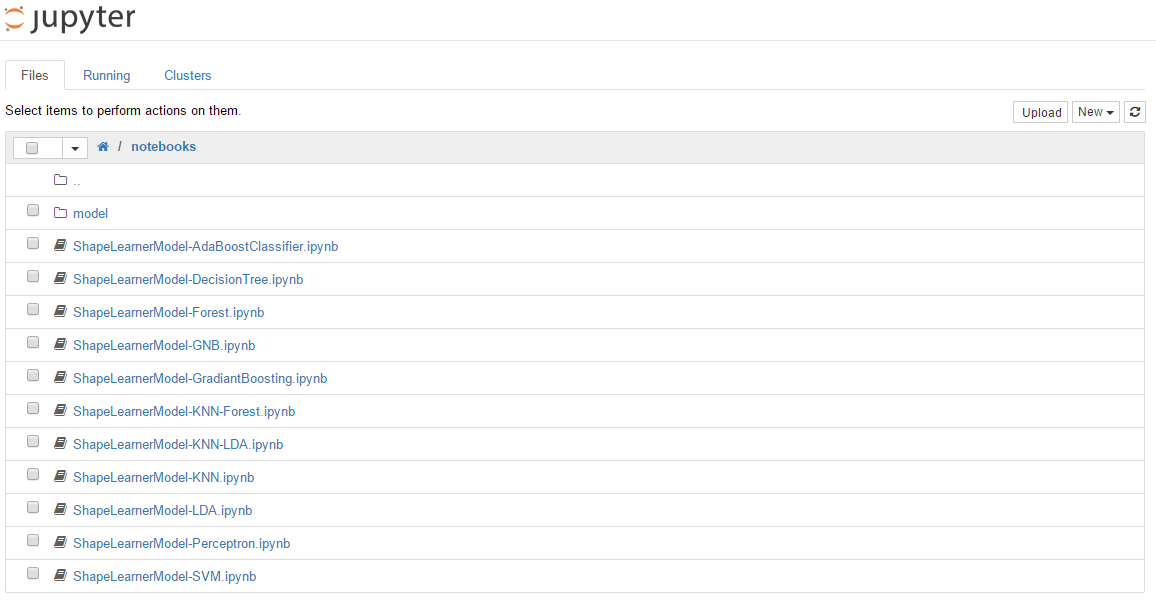
\includegraphics[width=18cm]{machineLearningAlgorithms.png}
	\caption{La totalité des algorithmes d'apprentissage automatique testés.}\label{image.MLListe} 
\end{figure}

Je regrette cependant ne pas avoir pu passer suffisamment de temps pour explorer toutes les pistes que j'avais pour améliorer le pourcentage de réussite. J'ai dû me contenter du résultat certes satisfaisant mais pouvant être très certainement amélioré.

L'algorithme donnant le meilleur résultat est le celui des \textit{k-plus-proches-voisins ou KNN (K-Nearest-Neighbors)} de la librairie Python : \textbf{\textit{Scikit-learn}}. J'ai obtenue le meilleur résultat en prenant les paramètres suivants :

\begin{itemize}
	\item \textbf{neighbors =}  53
	\item \textbf{weights =}  distance
	\item autres paramètres = valeur par défaut
\end{itemize}

\begin{center}
\textbf{On obtient un résultat de classification quasiment instantané avec une précision de l'ordre de 50\%.}
\end{center}

La valeur élevée du nombre de voisins peut s'expliquer par le fait que chaque pièce de la base de connaissance est représentée par environ 70 photos selon un grand nombre d'angles. Un nombre faible de voisins correspondant serait donc peu pertinent.

Dans la même idée, les poids des plus proches voisins ne sont pas uniformes mais fonction de l'inverse de la distance afin de fortement privilégier une grande ressemblance au détriment d'une faible correspondance.

Les données d'apprentissage qui sont en entrée de l'algorithme sont les \textit{\textbf{métadonnées}} des ShockGraphs générés. Par exemple, le nombre de nœuds, le nombre d'arêtes, le nombre d'arêtes par nœud, la taille de la boite englobante de l'objet ...

\subsubsection{ShapeLearner - PredictionAPI - Utilité ?}

La prédictionAPI sert de \textbf{filtre} afin de réduire le champs des possibles. Ainsi au lieux de comparer la pièce candidate à la totalité des pièces en base de connaissance, nous pouvons uniquement la comparer aux N-plus-probables. Ce qui aura pour effet de considérablement raccourcir le temps de traitement. L'objectif de la PredictionAPI n'est pas de fournir un résultat absolu mais d'éliminer les classes d'objets qui semblent sans rapport.

\subsubsection{ShapeLearner - PredictionAPI - Comment améliorer la précision ?}

Il est plus qu'envisageable qu'une étude plus approfondie aurait pu permettre de meilleurs résultats. J'aurais par exemple voulu avoir le temps de tester les réseaux de neurones multi-couches de manière plus poussée. Il semblerait que ces derniers soit particulièrement efficaces dans le domaine de la vision par ordinateur.

J'aurais également voulu avoir un peu plus de temps pour tester diverses combinaisons de modèle d'apprentissage. Pratique qui semble considérablement améliorer les résultats.

\subsection{Résultat finaux - ShapeLearnerAPI}

A l'heure où j'écris ce rapport, nous n'avons pas encore été en mesure d'effectuer les test finaux d'exécution du plugin ShapeLearnerAPI et de comparaison avec une base de test établie correctement. Cependant nous pouvons avancer des résultats très encourageant. La méthode affiche une précision qui avoisine les 70\% de réussite en temps suffisamment court pour être acceptable.

\subsection{Schéma de l'API}

 \begin{figure}[H]
    \centering
    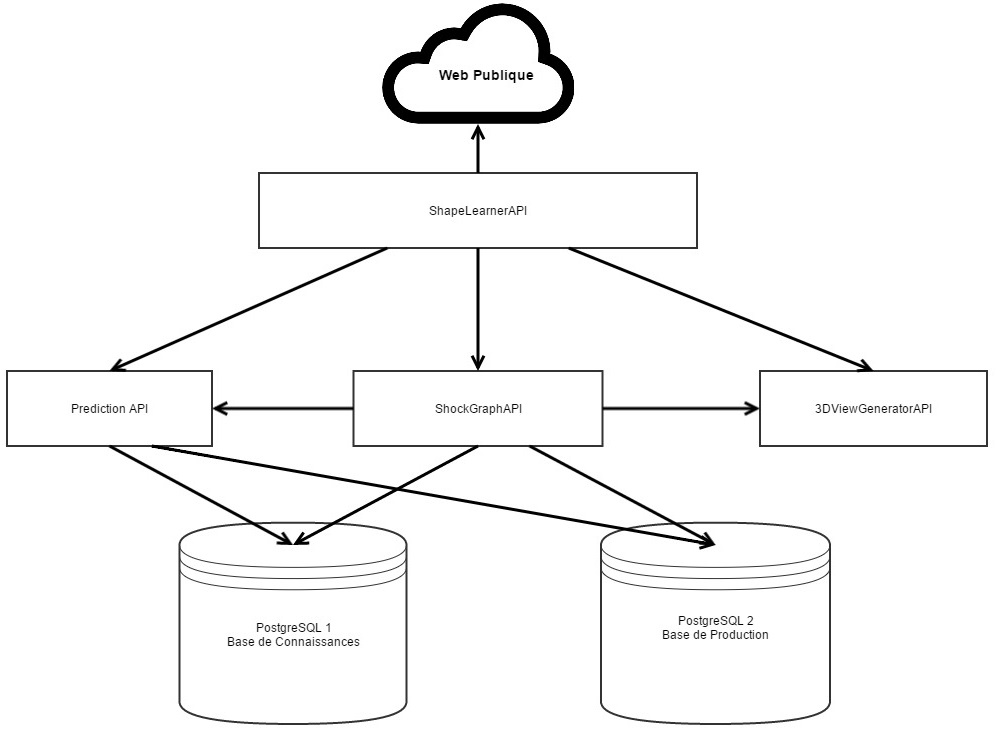
\includegraphics[width=18.7cm]{shapelearnerapi.jpg}
	\caption{Schéma interne côté serveur de ShapeLearnerAPI.}\label{image.ShapeAPIScheme} 
\end{figure}

\clearpage